\chapter{Methodology}
This methodology is divided into two sections: the method by which we simulated falls to acquire data to train our algorithm, and the method by which we created and evaluated our fall detection system.

\section{Participants}
Nine volunteers were involved in this experiment (all males). Participants had a median age of 21 (mean 26.5, min. 19, max. 49). All participants were sampled from the general population of an educational institution in the Greater Toronto Area in Ontario, Canada. Participants were recruited by a set of posters posted at various locations throughout the campus. The recruitment message did not disclose the purpose of the experiment but described the task as fun. The message indicated that each volunteer would receive compensation for his/her time and that volunteering would be a contribution to the advancement of science.


\section{Simulated Fall Study}
Unlike many areas of Machine Learning, where there is currently a rapidly growing number of datasets for scientists to explore deep learning and conduct research in machine learning, there are very few datasets for falls and none for falls of seniors. We found three public fall datasets:

\begin{enumerate}
    \item Multiple Cameras Fall Dataset \cite{Auvinet2011} contains 24 scenarios recorded with 8 video cameras from different perspectives in a room. The first 22 scenarios contain a fall and activities of daily living, the last 2 ones contain only ADL events.
    \item UR Fall Detection Dataset \cite{Kwolek2014} contains 30 falls and 40 activities of daily life activities. Fall events were recorded by 2 Microsoft Kinect cameras while non-fall events were recorded by only one device and an accelerometer.
    \item The Fall Detection Dataset \cite{Antoine2013} is a dataset in realistic video surveillance data recorded by a single camera. This dataset consists of 191 labeled videos at 25 FPS and 320x240 resolution, representing the fall-down position in the video sequence. This dataset is characterized by its multiple scenarios, including home, coffee room, office and lecture room, which can better test the robustness of fall detection algorithms.
\end{enumerate}


The \textit{Multiple Cameras Fall Dataset} has an extreme fisheye view in all videos which distorts the images; the resolution in the last two (\textit{UR Fall Detection} and the \textit{Fall Detection Dataset}) is very low. Unfortunately, these limitations prohibited us from using them in our study. Furthermore, these datasets did not include any aids (i.e., canes, walkers, etc.) that a senior would typically have, especially if s/he has balance issues. Consequently, this first portion of our methodology is a simulated fall dataset collection process.


In order to train our machine learning model, we created video footage of various falling and non-falling scenarios in a safe controlled environment as done by our young participants as it would not be appropriate to subject elderly people to simulated falls. A large crash mat was used to ensure the safety of the participants as they performed the prescribed routine. Each participant performed 7 different fall types and each fall-type was repeated 2 times. Thus, each young adult performed 14 falls. All gave written informed consent and the educational institution’s Research Ethics Board approved the protocol. Each participant was instructed to perform the following protocol while being video recorded:


\subsection{Non-fall scenarios:}
 \begin{itemize}
    \item Rising up from a chair (sitting position to a standing position),
    \item Sitting down in a chair from standing position,
    \item Walking around a desk in a large circle,
    \item Walking around in a large circle, towards and away from the camera,
    \item Walking around in a large circle with a cane, towards and away from the camera,
    \item Walking around in a large circle with a walker, towards and away from the camera.
\end{itemize}


\subsection{Fall scenarios:}
 \begin{itemize}
      \item Fall while initially leaning with a hand on a desk (e.g., simulating falling beside a counter in a kitchen for instance),
      \item Falling beside a desk,
      \item Falling from behind a desk,
      \item Stumbling backwards onto the ground after a perceived loss of balance,
      \item Falling forward from a chair after standing up,
      \item Falling to the side with canes, and lastly,
      \item Falling to the side with walkers.
\end{itemize}


More variety in video data from a diverse collection of angles has been shown to improve accuracy in machine learning models \cite{Auvinet2011, Kwolek2014, Antoine2013}.  Hence, all data collected was taken at multiple angles for filming. As for walking in a large circle, this was to have a variety of far away and close-ups of people relative to the camera while affording multiple perspectives and gait data collection.  This also was based on best practices for machine learning researchers curating their own image datasets \cite{Auvinet2011, Kwolek2014, Antoine2013}.  The use of the equipment (i.e., a cane and a walker), was incorporated into the protocol to better simulate walking patterns, gait, balance issues and appearances of seniors who likely use such aids, especially if they are at high risk for falling.  The non-fall scenarios were filmed to create a comprehensive fall dataset and enabled extensive training, validation and testing of our ML models.

A total of 235 videos were collected, with 115 being non-fall scenarios, and 120 being fall scenarios, collectively representing 36.4 minutes of footage. Each participant had on average 26 videos of their own actions, and the total data from all participants were used to train our ML models. Using conventional ML practices, 80\% of the video data was used for training and 20\% was for testing our models. Figure ~\ref{fig:falls} presents a) a participant falling forward, b) a participant falling backwards onto the mat, and c) a participant using a cane and falling to the side.

\begin{figure}
  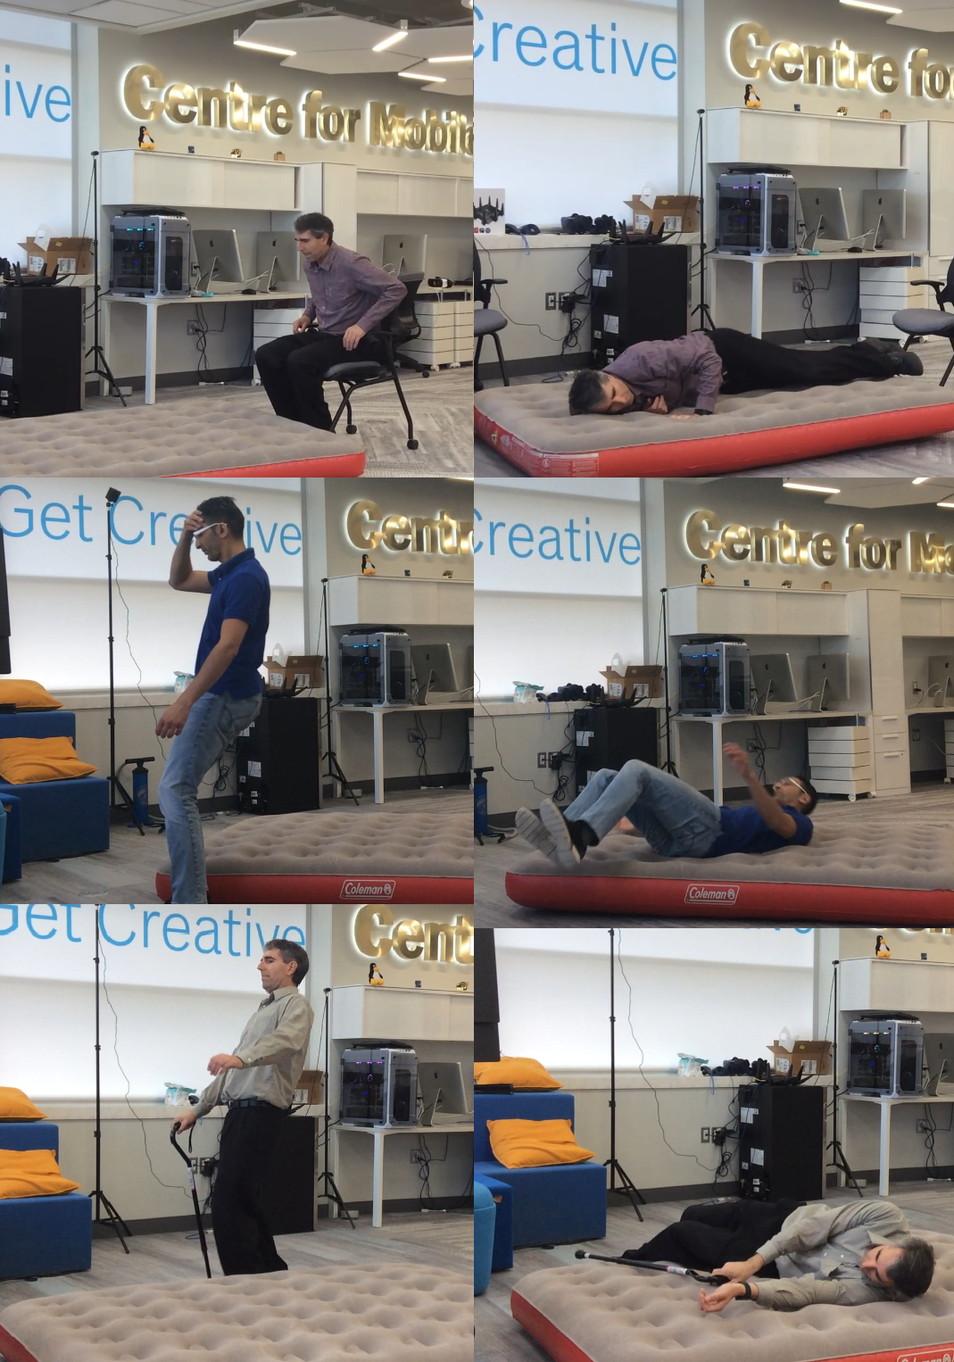
\includegraphics[width=\linewidth]{falls}
  \caption{A participant falling forward (a), a participant stumbling backward (b), and a participant using a cane and falling sideways (c).}
  \label{fig:falls}
\end{figure}


\section{Design}

In this section, we describe the process we followed to build a machine learning model that can detect falls. The machine learning model that fits this need is a logistic regression model that is based on a supervised classification algorithm. As shown in Figure ~\ref{fig:mlmodel4falldetection}, our model is defined as following:


\begin{figure}
  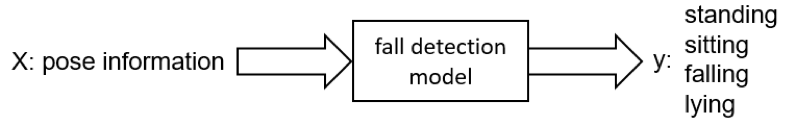
\includegraphics[width=\linewidth]{mlmodel4falldetection}
  \caption{Machine Learning Model for Fall Detection.}
  \label{fig:mlmodel4falldetection}
\end{figure}

 \begin{itemize}
        \item Input features (X): the input needed for our fall detection model are the keypoint positions that identify the pose of a single person.
        \item Target variable (y): the output of our model is a class that predicts the state of the person in the video (based on the input features). We restricted the classes in our model to four different classes: \textit{standing, sitting, falling} and \textit{lying}. During the initial stages of our ML research in creating a fall detection model, we included many other classes that were being tracked too, such as \textit{running, stretching, crouching,} etc. but these were removed from our output class to make the detection problem simpler. Instead, we used two classes only (\textit{Falling, Not Falling}), and discovered that having a limited amount of variation would help our history model (as described in section 3.3.3) to learn when determining a fall state.

\end{itemize}


Figure ~\ref{fig:mainpipeline} shows the overall process we followed to build our fall detection model using ML and human pose estimation. We describe the main steps and the choices we made in the following sections.

\begin{figure}
  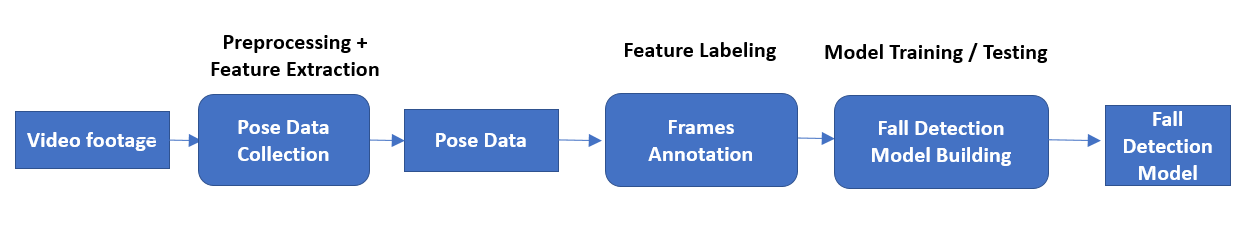
\includegraphics[width=\linewidth]{mainpipeline}
  \caption{Main Pipeline Used to Build a Fall Detection Algorithm Using ML and Human Pose Estimation.}
  \label{fig:mainpipeline}
\end{figure}



\subsection{Pose Data Collection}

In order to get pose information from a person in a video, we made use of two open-source libraries that can be used to estimate the pose of a person in an image or a video by estimating where key body joints are. The two libraries we used are PoseNet \cite{posenet2019} and OpenPose \cite{RN1003}. PoseNet is developed under MIT licence. It provides a lightweight implementation that uses TensorFlow JavaScript that runs in a web browser \cite{posenet2019}. With this implementation, PoseNet is able to detect 17 pose keypoints in a single image. OpenPose is a more accurate pose detection package that is developed under an academic and non-profit, non-commercial use only. It is written in C++ using OpenCV and Caffe. It enables the detection of up to 135 keypoints for one person in a single image.


We decided that the fall detection system would first require a data collection script to retrieve the pose data from a video regardless of using PoseNet or OpenPose. This pose data provided the input features to build the model. We wrote two different data collector implementations for this process (one for each library). The data, which represents keypoint information about positions of specific body parts on the people in the videos, was saved in JSON format for the OpenPose system and CSV format for the PoseNet system.


\subsection{Frames Annotation}


In order to train and build the models for each of the fall detection systems, we created ground truth datasets by tagging each frame of training videos fed through the data collector as a specific pose. We labeled every frame that contains pose data to one of our pre-defined classes: \textit{standing, sitting, lying down, or falling}. These annotated poses were then compiled into a list of frame-by-frame pose tags, which, when reaching a certain threshold, was considered to be a full list. For the OpenPose fall system, the threshold was 30 frames, and for PoseNet it was 25 frames. These numbers were determined over the course of evaluating what frame count produces the most accurate fall detection results.


\subsection{Fall Detection ML Model Building}

In this process, we used the labeled pose data we collected to build the fall detection machine learning model. Our model builder generates two different models: the first of which is based on frame-by-frame analysis and the second uses a novel frame history analysis technique. These two models are shown in Figure ~\ref{fig:historymodel}.




The first model allows prediction of one frame’s state (e.g. class), such as whether someone is \textit{standing, falling, sitting, or lying down} in a frame of video. A history analysis model allows determination of an estimated frame state for a series of frames. This second model takes in the pose estimates from the frame-by-frame prediction model’s output, in a list of 25 or 30 frame state predictions, depending on the fall system being used (OpenPose or PoseNet). By looking at the past \textit{‘frame state history’} in the last few seconds of the video that was already analyzed by the first machine learning model, the second model is able to make an estimation on what state a given person is in considering past information rather than simply what is visually observable in one specific frame in the video. We explored this approach because during testing, it became clear that fall states could not be determined from one frame of a video alone – to accurately predict a real fall, one needs to know how fast the person is moving from frame to frame, and in what way. The second model we created is based on \textit{frame history analysis} in order to address this problem.



Our novel frame history analysis technique equips the system to consider the person’s position in the past as it relates to the current frame being analyzed. The frame history model’s output is used to determine the final test results for both fall detection systems.


The PoseNet based model was made using \textit{nodesvm} \cite{RN1003}, while the OpenPose based model was made with \textit{scikit-learn} \cite{posenet2019}. Many OpenPose models were created through experimentation using scikit-learn’s algorithms, namely, Linear SVC, Naïve Bayes, SVC, and Kernel Approximation (see Figure ~\ref{fig:openposetrainingmodels}). Ultimately, the results of the experimentation were used to compare our best OpenPose model with the best PoseNet model.


\begin{figure}
  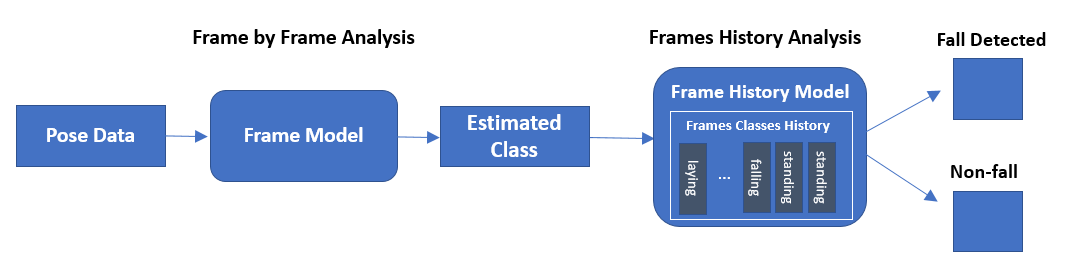
\includegraphics[width=\linewidth]{historymodel}
  \caption{Fall Detection Model Building Process.}
  \label{fig:historymodel}
\end{figure}



\begin{figure}
  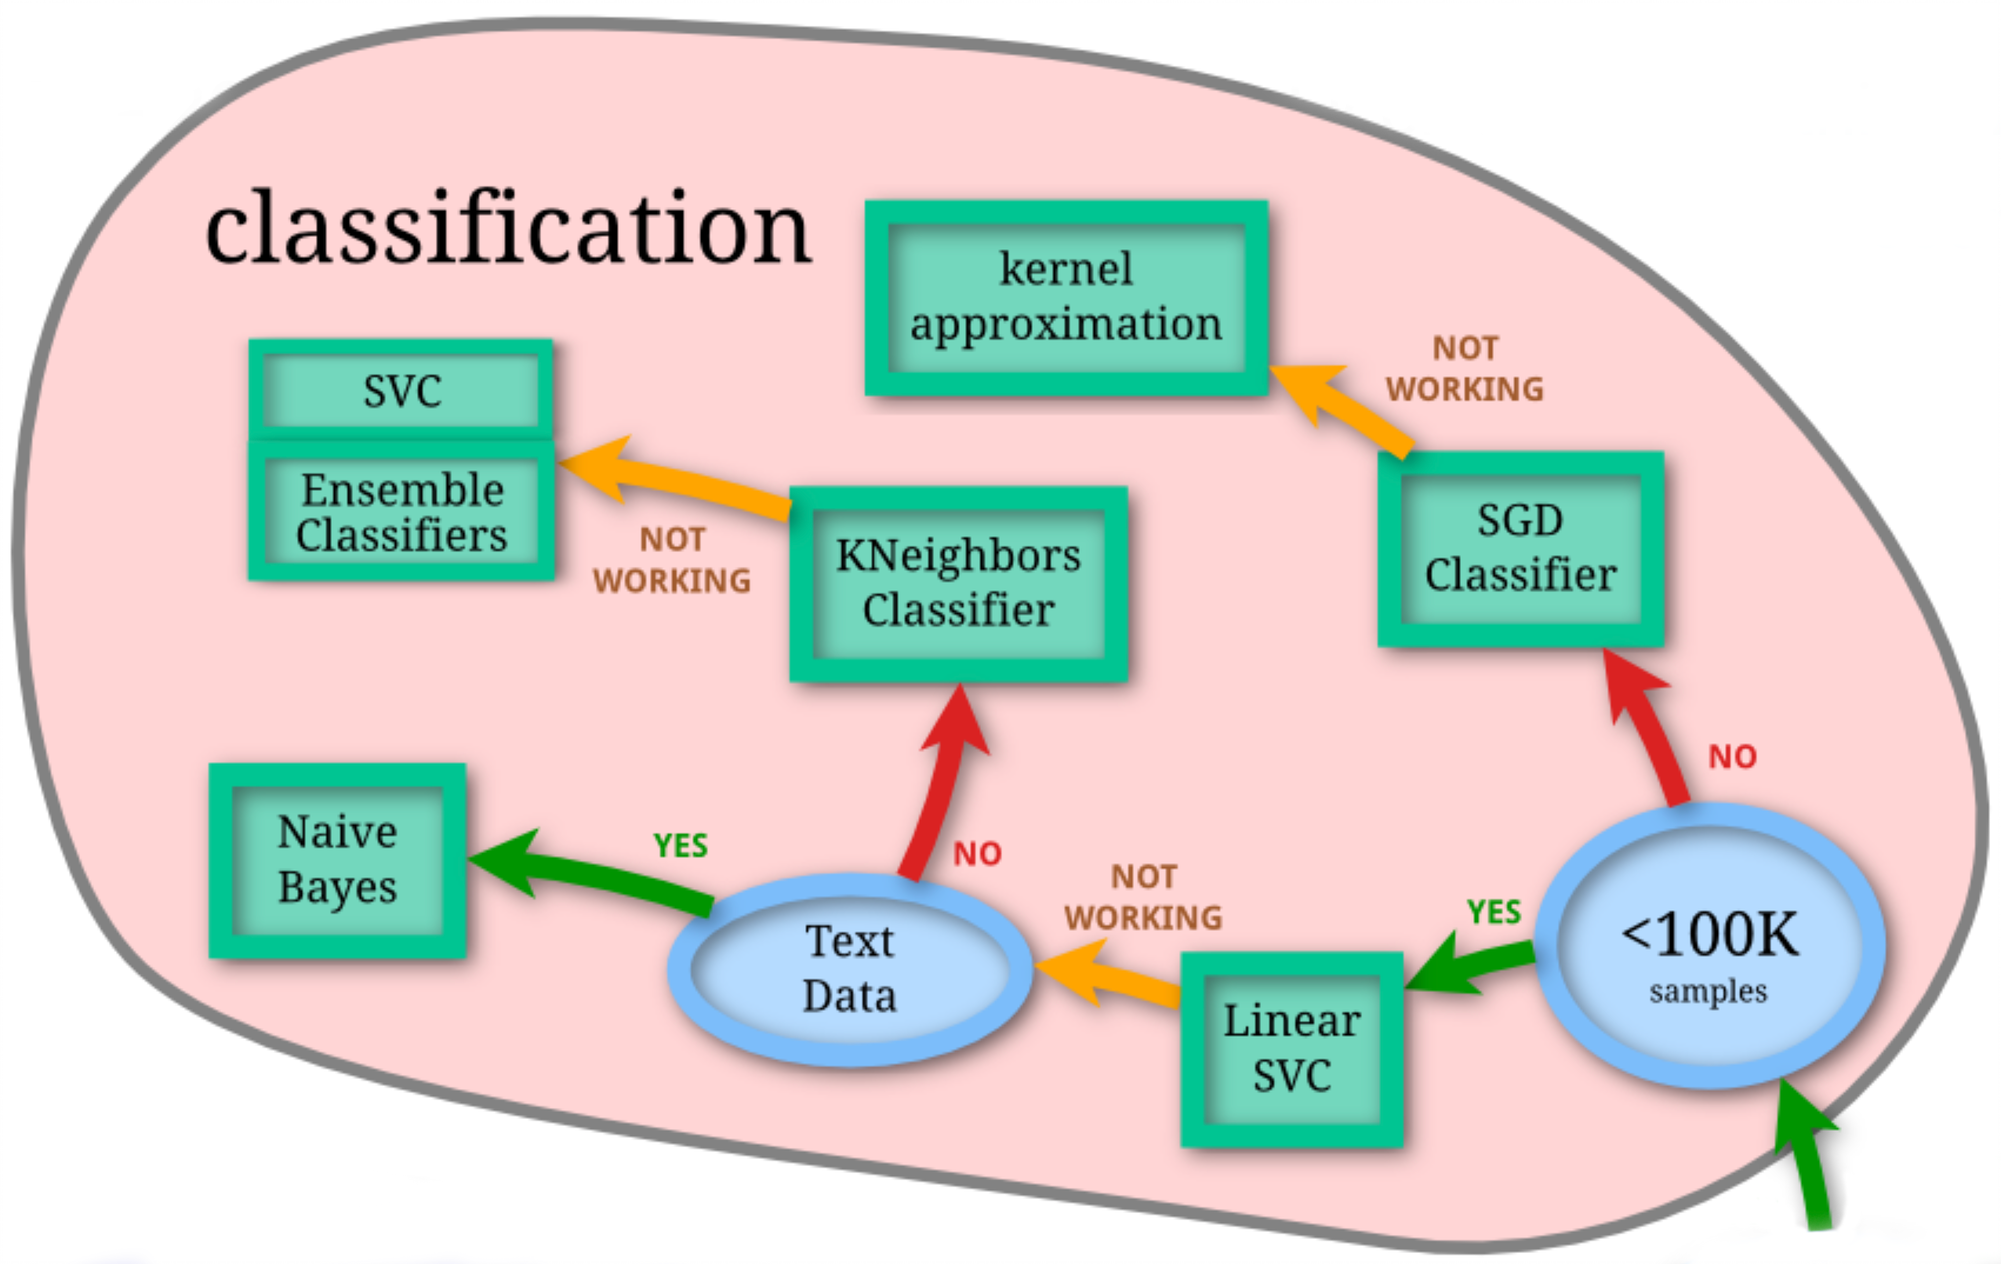
\includegraphics[width=\linewidth]{openposetrainingmodels}
  \caption{Scikit-learn Classification Road-Map.}
  \label{fig:openposetrainingmodels}
\end{figure}


The fall detection model building process generated model files that classify pose data into \textit{fall} or \textit{no-fall} categories. We then created a predictor script that uses these models to make predictions about video pose data, provided by PoseNet or OpenPose, to ascertain about whether a fall is detected in a given video footage.


In order to generate statistics on the performance of both fall detection systems using either PoseNet or OpenPose, models were built for each system based on 193 videos of the total 235 videos (80\% of all videos were used as training videos (randomly shuffled). 20\% of the remaining videos were used for testing.  These models were used with the predictor script on each system to produce predictions based on data gathered through the data collector scripts on each fall system. Videos were placed into different datasets based on which person was featured in the videos, so there were 9 groups of videos based on the 9 participants. Once prediction data were gathered, the results were organized into confusion matrices where true positives represent a true fall detection (i.e., ground truth – the frame was tagged with the person \textit{falling}).



\section{Analysis}

The following types of quantitative analysis were performed: 1) evaluating and refining the classifier using standard machine learning evaluation tools; and 2) determining the accuracy of the classifier using statistical tools.


\begin{enumerate}
    \item Computing confusion matrices: Compare the classifier’s accuracy at predicting a fall using actual video analysis as ideal. Confusion matrices and the associated measures (Accuracy, Precision and Sensitivity) are commonly used in the evaluation of machine learning algorithms, please see: \cite{Elkan12evaluatingclassifiers, Forman2010, Kohavi1998, lu2004, Hamilton2011}. Statistics for each participant for each classifier model was collected on:

    True Positives (TP): \textit{(classifier correctly detected a fall);}


    True Negatives (TN): \textit{(classifier correctly selected “Not a fall”);}


    False Negatives (FN): \textit{("Didn't identify a fall when it should have");}


    False Positives (FP): \textit{(“False Alarm”—classifier said it was a fall when it shouldn’t have);}


    \[Accuracy =\frac{TP + TN}{TP + TN + FN + FP}\]
    \[Precision =\frac{TP}{TP + FP}\]
    \[Sensitivity =\frac{TP}{TP + FN}\]
    \[Specificity =\frac{TN}{TN + FP}\]
    \[Fall  Positive  Rate (FPR) =\frac{FP}{FP + TN}\]
    \[FScore =\frac{2*TP}{2*TP + FP + FN}\]

    \item Calculating standard descriptive statistics on the confusion matrix data for the entire group including minimum, maximum, mean, median, standard deviation, accuracy, precision, and sensitivity.
\end{enumerate}


